\section{Дървета на извод}

\newcommand{\high}{\texttt{height}}
\newcommand{\leaves}{\texttt{leaves}}
\newcommand{\successor}{\texttt{succ}}

\tikzset{
  photon/.style={decorate, decoration={snake}, draw=black}
}

\mynote{Понятието дърво е едно от най-основните в информатиката и може да се дефинира по много различни начини, в зависимост от това за какви цели се използва. Тук на практика следваме \cite{nerode-shore}, защото е важно да имаме наредба между възлите на дървото.}
\begin{itemize}
\item
  За фиксирано $b \in \Nat$, ще разглеждаме думи $\alpha$ и $\beta$ над азбуката $\{0,1,\dots,b-1\}$.
\item
  С $\alpha \preceq \beta$ ще означаваме, че $\alpha$ е префикс на $\beta$, а с $\alpha \prec \beta$,
  че $\alpha$ е \emph{същински} префикс на $\beta$, т.е. $\alpha \preceq \beta\ \&\ \alpha \neq \beta$.
\item
  \index{наредба!лексикографска}
  Ще казваме, че $\alpha$ е лексикографски по-малка от $\beta$, което ще означаваме като $\alpha <_{\texttt{lex}} \beta$, ако
  \[(\exists i < \min\{|\alpha|,|\beta|\})[\ (\forall j < i)[\ \alpha[j] = \beta[j]\ ]\ \&\ \alpha[i] < \beta[i]\ ].\]
\item
  \index{дърво}
  \mynote{Всеки възел в дървото еднозначно се определя от пътя от възела до корена.}
  Непразното множество $T \subseteq \{0,1,\dots,b-1\}^\star$ се нарича {\bf дърво},
  ако $T$ е затворено относно префикси, т.е. $\texttt{Pref}(T) = T$.
  С други думи,
  \[(\forall \alpha)(\forall \beta)[\ \alpha \in T\ \&\ \beta \preceq \alpha\ \implies\ \beta \in T\ ].\]
  \mynote{При нас всички дървета са крайно разклонени.}
\item
  Нека да въведем следните означения:
  \begin{align*}
    & \high(T) \df \max\{\ \abs{\alpha}\ \mid\ \alpha \in T\ \} & \comment\text{височина}\\
    & \successor_T(\alpha) \df \{ \alpha i \mid \alpha i \in T\ \&\ i < b\} & \comment\text{наследниците на }\alpha\\
    & T_\alpha \df \alpha^{-1}(T) & \comment\text{поддървото на }\alpha\\
    & \leaves(T) \df \{ \alpha \in T \mid \successor_T(\alpha) = \emptyset \}. & \comment\text{листата на }T
  \end{align*}

  \begin{figure}[H]
    \centering
    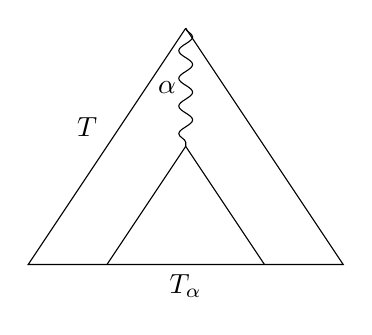
\begin{tikzpicture}
      \coordinate (A) at (0,0);
      \coordinate (B) at (-2,-3);
      \coordinate (C) at (2,-3);
      \coordinate (D) at (0,-1.5);
      \coordinate (E) at (-1,-3);
      \coordinate (F) at (1,-3);
      \draw (A) -- node[above left]{$T$} (B) -- node[below]{$T_\alpha$}(C) -- (A);
      \draw (D) -- (E);
      \draw (D) -- (F);
      \draw [photon] (A) -- node[left]{$\alpha$} (D);
    \end{tikzpicture}
    \caption{Поддърво $T_\alpha$ на $T$.}
  \end{figure}  
\item
  Нека фиксираме граматиката $G = (\Sigma,V,S,R)$.
  С всяко дърво $T$ ще асоциираме функцията $\lambda: T \to V \cup \Sigma \cup \{\varepsilon\}$.
  Нека положим $X_\alpha \df \lambda(\alpha)$.
\item
  \index{дърво на извод}
  \mynote{Също се нарича синтактично дърво. На англ. \emph{parse tree}.}
  Двойката $P = (T,\lambda)$ се нарича {\bf дърво на извод} съвместимо с $G$, ако са изпълнени свойствата:
  \begin{itemize}
  \item
    $T$ е крайно.
  \item
    Ако $\alpha i \in T$, то $\alpha j \in T$ за всяко $j < i$.
  \item
    Ако $\alpha \in T$ и $|\texttt{ext}_T(\alpha)| = k+1$, за някое $k \in \Nat$, то $X_\alpha \in V$,
    като имаме също така и 
    % Освен това, ако $\alpha_0,\dots,\alpha_k$ са всички думи от множеството $\texttt{ext}_T(\alpha)$
    % подредени във възходящ ред относно лексикографската наредба, то имаме, че:
    \mynote{С други думи,
      \[\lambda(\alpha)\to_G\lambda(\alpha 0)\cdots\lambda(\alpha k).\]}
    \[X_\alpha \to_G X_{\alpha 0} X_{\alpha 1} \cdots X_{\alpha k}.\] 
  \end{itemize}
\item
  За дървото на извод $P$, нека
  \[\texttt{root}(P) \df X_\varepsilon.\]
\item
  Нека $\alpha_0, \alpha_1,\dots,\alpha_k$ са всички думи от множеството $\leaves(T)$
  подредени във възходящ ред относно лексикографската наредба. Тогава 
  \[\texttt{yield}(P) \df X_{\alpha_0} X_{\alpha_1}\cdots X_{\alpha_k}.\]
\item
  \mynote{В \cite[стр. 123]{papadimitriou} дават рекурсивна дефиниция на дърво на извод.}
  Нека $P = (T,\lambda)$ е дърво на извод съвместимо с граматиката $G$.
  За всяко $\alpha \in T$, дефинираме $\lambda_\alpha:T_\alpha \to V \cup \Sigma \cup \{\varepsilon\}$ като
  \[\lambda_\alpha(\beta) \df \lambda(\alpha \cdot \beta).\]
\item
  Нека $P = (T,\lambda)$ и $\alpha \in T$. Тогава
  \[P_\alpha \df (T_\alpha, \lambda_\alpha).\]
\end{itemize}

\begin{example}
  Да разгледаме граматиката $G$, където правилата са следните:
  \begin{align*}
    & S \to aS\ |\ aSc\ |\ B\\
    & B \to bB\ |\ bBc\ |\ \varepsilon.
  \end{align*}
  Вече знаем, че $\L(G) = \{a^nb^kc^\ell \mid n+k\geq \ell\}$.
  Да разгледаме дървото на извод $P = (T, \lambda)$, където:

  \begin{framed}
    \begin{figure}[H]
    \qtreecenterfalse
    \Tree [.$\varepsilon$ $0$ [.$1$ $10$ [.$11$ [.$110$ $1100$ [.$1101$ $11010$ ] $1102$ ] ] $12$ ] ]
    \hskip 0.4in
    $\stackrel{\lambda}{\Rightarrow}$
    \hskip 0.4in
    \Tree [.S a [.S a [.S [.B b [.B $\varepsilon$ ] c ] ] c ] ]
    \caption{Дърво на извод за думата $aabcc$.}      
    \end{figure}
  \end{framed}

  Имаме, че:
  \begin{itemize}
  \item
    $\high(T) = 5$;
  \item
    $\leaves(T) = \{0, 10, 1100, 11010, 1102, 12\}$;
  \item
    $\texttt{yield}(P) = aab\varepsilon cc = aabcc$.
  \item
    $\successor_T(110) = \{1100, 1101, 1102\}$;
  \item
    $\lambda(\varepsilon) = S$;
  \item
    $\lambda(0) = a$, $\lambda(1) = S$;
  \item
    Ясно е, че $\lambda(\varepsilon) \to_G \lambda(0)\lambda(1)$;
  \item
    $\lambda(10) = a$, $\lambda(11) = S$, $\lambda(12) = c$;
  \item
    Ясно е, че $\lambda(1) \to_G \lambda(10)\lambda(11)\lambda(12)$;
  \item
    $\lambda(110) = B$;
  \item
    Ясно е, че $\lambda(11) \to_G \lambda(110)$;
  \item
    $\lambda(1100) = b$, $\lambda(1101) = B$, $\lambda(1102) = c$;
  \item
    Ясно е, че $\lambda(110) \to_G \lambda(1100)\lambda(1101)\lambda(1102)$;
  \item
    $\lambda(11010) = \varepsilon$;
  \item
    Ясно е, че $\lambda(1101) \to_G \lambda(11010)$;
  \end{itemize}
  От всичко по-горе следва, че $P = (T,\lambda)$ е дърво на извод за думата $aabcc$ в граматиката $G$.  
\end{example}

\begin{problem}
  Докажете, че:
  \begin{itemize}
  \item
    $T = \texttt{Pref}(\leaves(T))$;
  \item
    $T = T' \iff \leaves(T) = \leaves(T')$.
  \end{itemize}
\end{problem}

\begin{lemma}
  Нека $T \subseteq \{0,\dots,b-1\}^\star$ е крайно дърво. Тогава
  \[ |\leaves(T)| \leq b^{\high(T)}.\]
\end{lemma}
\begin{proof}
  Индукция по $\high(T)$.
  \begin{itemize}
  \item
    Нека $\high(T) = 0$. Тогава е ясно, че $|\leaves(T)| = |\{\varepsilon\}| = 1 \leq b^0$.
  \item
    Нека $\high(T) > 0$.
    За всяко $a \in T$ е ясно, че $\high(T_a) < \high(T)$. Тогава:
    \mynote{В този случай имаме, че $\leaves(T) = \bigcup_{a\in T} (\{a\}\cdot \leaves(T_a))$. Тук гледаме на $a$ и $b$ от една страна като букви в азбука, но и като числа.}
    \begin{align*}
      |\texttt{leaves}(T)| & = \sum_{a \in T}|\texttt{leaves}(T_a)|\\
                           & \leq \sum_{a \in T} b^{\high(T_a)} & \comment\text{от \IndHyp}\\
                           & \leq \sum_{a < b} b^{\high(T_a)}\\
                           & \leq \sum_{a < b} b^{\high(T) -1} & \comment \high(T_a) \leq \high(T)-1 \\
                           & = b^{\high(T)}.
    \end{align*}
  \end{itemize}
\end{proof}

\begin{framed}
  \begin{corollary}
    \label{cor:tree:upper-bound}
    Нека $P = (T,\lambda)$ е дърво на извод съвместимо с $G$. Тогава
    \[|\texttt{yield}(P)| \leq b^{{\high}(P)}.\]
  \end{corollary}
\end{framed}
\begin{proof}
  Следва директно от горното твърдение след като съобразим, че
  \[|\texttt{yield}(P)| \leq |\leaves(P)|.\]
\end{proof}

\begin{framed}
  \begin{lemma}
    Ако $X \derive{\star}_G \beta$, то $X \yield{\star}_G \beta$.
  \end{lemma}  
\end{framed}
\begin{proof}
  Индукция по дължината на извода $X \derive{\ell} \beta$.
  \begin{itemize}
  \item
    $\ell = 0$, т.е. $X \derive{0} X$.
    Тогава е ясно, че $X \yield{\star} X$.
  \item
    \mynote{Знаем, че $k < b$.}
    Нека $\ell > 0$ и $X \derive{\ell} \beta$.
    Според правилата на извод в граматика имаме извода
    \[X \to_G X_0X_1\cdots X_k \derive{\ell-1} \beta.\]
    От \Proposition{grammar:divide} знаем, че съществува разбиване на $\beta$ на $k+1$ части, така че:
    \begin{itemize}
    \item
      $\beta = \beta_0 \cdots \beta_{k}$;
    \item
      $X_i \derive{\ell_i} \beta_i$, за всяко $i = 0,\dots,k$;
    \item
      $\ell-1 = \sum^k_{i=1} \ell_i$.
    \end{itemize}
    От \IndHyp имаме, че $X_i \yield{\star} \beta_i$ за $i \leq k$.
    Получаваме следното:
    \begin{prooftree}
      \AxiomC{$\vdots$}
      \LeftLabel{\scriptsize{\IndHyp}}
      \UnaryInfC{$X_i \yield{\star} \beta_i \text{ за }i \leq k$}
      \AxiomC{$X \to_G X_0\cdots X_k$}
      \BinaryInfC{$X \yield{\star} \underbrace{\beta_0\cdots\beta_k}_{\beta}$}
    \end{prooftree}
  \end{itemize}
\end{proof}

\begin{framed}
  \begin{lemma}
    Ако $X \yield{\star}_G \gamma$, то $X \derive{\star}_G \gamma$.
  \end{lemma}
\end{framed}
\begin{proof}
  Индукция по височината $\ell$ на дървото на извод за $X \yield{\ell} \gamma$.
  \begin{itemize}
  \item
    Нека $\ell = 0$. Това означава, че $X \yield{0} X$. Ясно е, че $X \derive{\star} X$.
  \item
    Нека $\ell > 0$. Тогава имаме следното:
    \begin{prooftree}
      \AxiomC{$X \to_G X_1\cdots X_n$}
      \AxiomC{$X_i \yield{\ell_i} \gamma_i\text{ за }i=1,\dots,n$}
      \RightLabel{\scriptsize{($\ell = 1 + \max\{\ell_1,\dots,\ell_n\})$}}
      \BinaryInfC{$X \yield{\ell} \gamma_1\cdots\gamma_n$}
    \end{prooftree}
    Тогава от И.П. получаваме, че за всяко $i < k$ е изпълнено $X_i \derive{\star} \gamma_i$.
    Получаваме, че:
    \begin{prooftree}
      \AxiomC{$X \to_G X_0 \cdots X_{k-1}$}
      \AxiomC{$\vdots$}
      \RightLabel{\scriptsize{\IndHyp}}
      \UnaryInfC{$X_i \derive{\star} \gamma_i\text{ за }i<k$}
      \UnaryInfC{$X_0 \cdots X_{k-1} \derive{\star} \gamma_0\cdots\gamma_{k-1}$}
      \BinaryInfC{$X \derive{\star} \underbrace{\gamma_0\cdots\gamma_{k-1}}_{\gamma}$}
    \end{prooftree}
  \end{itemize}
\end{proof}

\begin{framed}
\begin{theorem}
  Нека $G$ е произволна безконтекстна граматика.
  Тогава $\alpha \in \L(G)$ точно тогава, когато съществува дърво на извод $P$, съвместимо с $G$, с корен $S$ за думата $\beta$.
\end{theorem}  
\end{framed}



\begin{problem}
  Нека $P = (T,\lambda)$ е дърво на извод за думата $\alpha \in (V\cup\Sigma)^\star$ в граматиката $G$.
  Докажете, че съществува извод
  \mynote{Ясно е, че $\ell < b^{\high(T)}$.}
  $X_\varepsilon \stackrel{\ell}{\to}_G \alpha$, където
  \[\ell \leq \sum_{i < \high(T)}b^i.\]
\end{problem}

\begin{problem}
  Нека $P = (T,\lambda)$ е дърво на извод съвместимо с $G$.
  Докажете, че ако $\alpha \preceq \beta$, то $\texttt{yield}(T_\beta)$ е инфикс на $\texttt{yield}(T_\alpha)$.
\end{problem}
\begin{hint}
  Нека $\beta = \alpha \cdot \gamma$. Тогава имаме следното дърво:
  
  \begin{figure}[H]
    \centering
    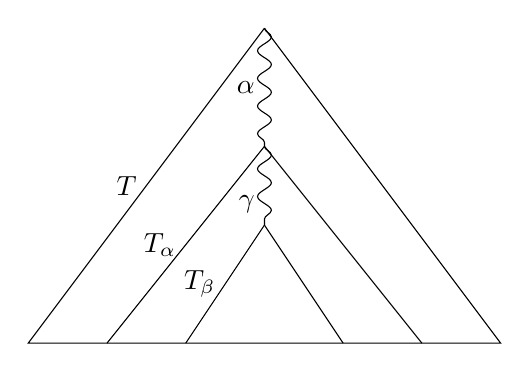
\begin{tikzpicture}
      \coordinate (A) at (0,0);
      \coordinate (B) at (-3,-4);
      \coordinate (C) at (3,-4);
      \coordinate (D) at (0,-1.5);
      \coordinate (E) at (-2,-4);
      \coordinate (F) at (2,-4);
      \coordinate (G) at (0,-2.5);
      \coordinate (H) at (-1,-4);
      \coordinate (I) at (1,-4);
      
      \draw (A) -- node[left]{$T$} (B) -- (C) -- (A);
      
      \draw (D) -- node[left]{$T_\alpha$}(E);
      \draw (D) -- (F);
      
      \draw (G) -- node[left]{$T_\beta$}(H);
      \draw (G) -- (I);
      
      \draw [photon] (A) -- node[left]{$\alpha$} (D);
      \draw [photon] (D) -- node[below left]{$\gamma$} (G);
    \end{tikzpicture}
    \caption{}
  \end{figure}
\end{hint}

\begin{problem}
  Нека $P = (T,\lambda)$ и $P' = (T',\lambda')$ са дървета на извод съвместими с граматиката $G$ и нека
  имаме думи $\omega_1, \omega_2 \in \Sigma^\star$, за които
  \mynote{Това означава, че съществува $\alpha \in T$, за което $\lambda(\alpha) = \texttt{root}(P') = \lambda'(\varepsilon)$.}
  \[\texttt{yield}(P) = \omega_1 \cdot \texttt{root}(P') \cdot \omega_2.\]
  Дефинираме $P'' = (T'',\lambda'')$ по следния начин:
  \begin{itemize}
  \item
    \mynote{Ясно е, че $\alpha \in T$ и $\alpha \in \alpha\cdot T'$, но понеже $X_\alpha = X'_\varepsilon$, то нямаме проблем.}
    $T'' \df T \cup \{\alpha\} \cdot T'$;
  \item
    Сега трябва да дефинираме функцията $\lambda'' : T'' \to V \cup \Sigma \cup \{\varepsilon\}$.
    
    $\lambda''(\gamma) \df
    \begin{cases}
      \lambda(\gamma), & \text{ако }\gamma \in T\\
      \lambda'(\beta), & \text{ако }\gamma = \alpha \cdot \beta\ \&\ \beta \in T'
    \end{cases}$

    \mynote{Тук трябва да сме внимателни, защото двата случая на дефиницията на $\lambda''$  се засичат за $\gamma = \alpha$.
      Понеже $\alpha \in \texttt{leaves}(T)$ и $\lambda(\alpha) = \lambda'(\varepsilon)$, то функцията $\lambda''$ е коректно дефинирана.}
  \end{itemize}
  \index{дърво на извод!конкатенация}
  Тогава $P''$ е дърво на извод съвместимо с граматиката $G$ и
  \[\texttt{yield}(P'') = \omega_1 \cdot \texttt{yield}(P') \cdot \omega_2.\]
  Нека в такъв случай да означаваме $P'' = P \odot P'$ и ще казваме, че $P''$ е конкатенацията на $P$ и $P'$.
  
  \begin{figure}[H]
    \begin{subfigure}[t]{0.5\textwidth}
      \centering
      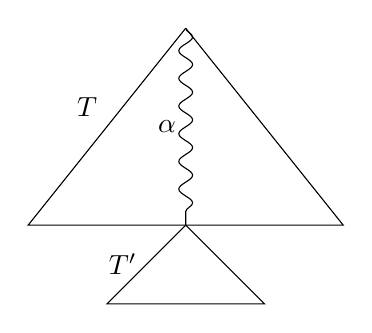
\begin{tikzpicture}
        \coordinate (A) at (0,0);
        \coordinate (B) at (-2,-2.5);
        \coordinate (C) at (2,-2.5);
        \coordinate (D) at (0,-2.5);
        \coordinate (E) at (-1,-3.5);
        \coordinate (F) at (1,-3.5);
        
        \draw (A) -- node[above left]{$T$} (B) -- (C) -- (A);
        \draw (D) -- node[left]{$T'$} (E) -- (F) -- (D);
        
        \draw [photon] (A) -- node[left]{$\alpha$} (D);
      \end{tikzpicture}
      \caption{Дървото $T''$}
      \end{subfigure}
      $\stackrel{\lambda}{\Rightarrow}$
      \begin{subfigure}[t]{0.5\textwidth}
        \centering
        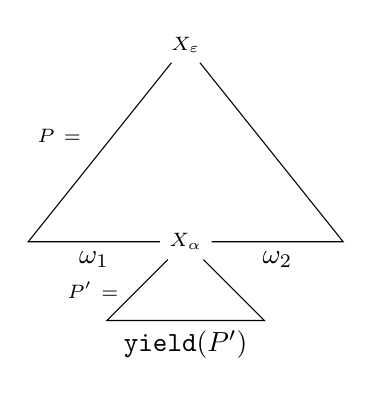
\begin{tikzpicture}
          \node (A) at (0,0) {${\scriptstyle X_\varepsilon}$};
          \coordinate (B) at (-2,-2.5);
          \coordinate (C) at (2,-2.5);
          \node (D) at (0,-2.5) {${\scriptstyle X_\alpha}$};
          \coordinate (E) at (-1,-3.5);
          \coordinate (F) at (1,-3.5);
          
          \draw (A) -- node[above left]{${\scriptstyle P\ =\ }$} (B) -- node[below]{$\omega_1$}(D) -- node[below]{$\omega_2$}(C) -- (A);
          \draw (D) -- node[left]{${\scriptstyle P'\ =\ }$}(E) -- node[below]{$\texttt{yield}(P')$}(F) -- (D);
          
          % \draw [photon] (A) -- node[left]{$\alpha$} (D);
        \end{tikzpicture}
        \caption{$P'' = P \odot P'$}
      \end{subfigure}
      \caption{Конкатенация на дървета}
    \end{figure}
  \end{problem}
  
  Сега да разгледаме частния случай, когато разгледаме $P$ вместо $P'$ в горните условия. Тогава имаме, че $X_\varepsilon = X_\alpha$.
  Дефинираме $n$-тата степен на дървото $P$ по следния начин:
  \begin{itemize}
\item
  $P^{(0)} \df (T_0,\lambda_0)$, където $T_0 = \{\varepsilon\}$ и $\lambda_0(\varepsilon) = \texttt{root}(P)$;
\item
  $P^{(n+1)} \df P^{(n)} \odot P$.
\end{itemize}

\begin{problem}
  Докажете, че $P \odot (P \odot P) = (P \odot P) \odot P$.
\end{problem}


\begin{problem}
  Докажете, че $P^{(n+k)} = P^{(n)} \odot P^{(k)}$.
\end{problem}

\begin{framed}
  \begin{problem}
    \label{prob:tree:iteration}
    Нека $\texttt{yield}(P) = \omega_1 \cdot \texttt{root}(P) \cdot \omega_2$, за някои думи $\omega_1, \omega_2 \in \Sigma^\star$.
    Докажете, че за всяко естествено число $i$ е изпълнено, че:
    \[\texttt{yield}(P^{(i)}) = \omega^i_1 \cdot \texttt{root}(P) \cdot \omega^i_2.\]
  \end{problem}
\end{framed}
\begin{hint}
  Картинката за $i = 2$ изглежда така:

  \begin{figure}[H]
    \begin{subfigure}[t]{0.5\textwidth}
      \centering
      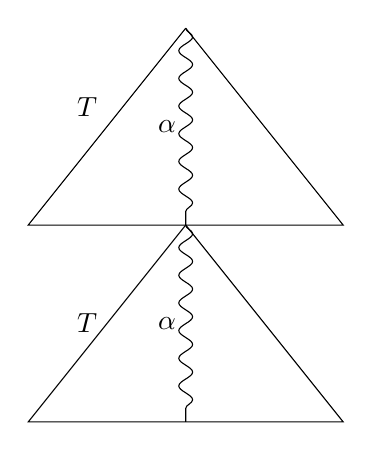
\begin{tikzpicture}
        \coordinate (A) at (0,0);
        \coordinate (B) at (-2,-2.5);
        \coordinate (C) at (2,-2.5);
        \coordinate (D) at (0,-2.5);
        \coordinate (E) at (-2,-5);
        \coordinate (F) at (2,-5);
        \coordinate (G) at (0,-5);
        
        \draw (A) -- node[above left]{$T$} (B) -- (C) -- (A);
        \draw (D) -- node[left]{$T$} (E) -- (F) -- (D);
        
        \draw [photon] (A) -- node[left]{$\alpha$} (D);
        \draw [photon] (D) -- node[left]{$\alpha$} (G);
      \end{tikzpicture}
      \caption{}
    \end{subfigure}
    $\stackrel{\lambda}{\Rightarrow}$
    \begin{subfigure}[t]{0.5\textwidth}
      \centering
      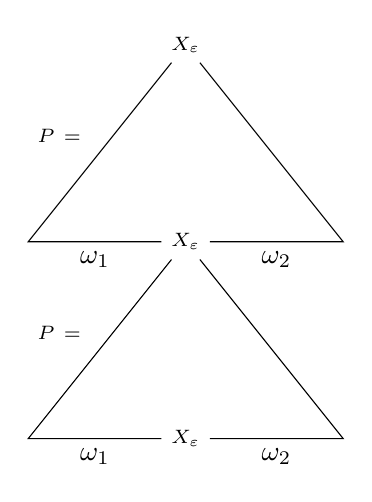
\begin{tikzpicture}
        \node (A) at (0,0) {${\scriptstyle X_\varepsilon}$};
        \coordinate (B) at (-2,-2.5);
        \coordinate (C) at (2,-2.5);
        \node (D) at (0,-2.5) {${\scriptstyle X_\varepsilon}$};
        \coordinate (E) at (-2,-5);
        \coordinate (F) at (2,-5);
        \node (G) at (0,-5) {${\scriptstyle X_\varepsilon}$};
        
        \draw (A) -- node[above left]{${\scriptstyle P\ =\ }$} (B) -- node[below]{$\omega_1$}(D) -- node[below]{$\omega_2$}(C) -- (A);
        \draw (D) -- node[above left]{${\scriptstyle P\ =\ }$}(E) -- node[below]{$\omega_1$} (G) -- node[below]{$\omega_2$} (F) -- (D);
      \end{tikzpicture}
      \caption{$\texttt{yield}(P^{(2)}) = \omega^2_1 \cdot \texttt{root}(P) \cdot \omega^2_2$}
    \end{subfigure}
    \caption{Степенуване на $P$.}
  \end{figure}
\end{hint}

\begin{problem}
  Нека $P = (T,\lambda)$ е дърво на извод съвместимо с граматиката $G$ и нека разгледаме думата $\alpha \in T$.
  % Дефинираме $P \setminus P_\alpha = (T',\lambda')$ по следния начин:
  Дефинираме $\uppercut{P}{\alpha} = (T',\lambda')$ по следния начин:
  \begin{itemize}
  \item
    \mynote{Съобразете, че $\alpha \in \texttt{front}(T')$.}
    $T' = T \setminus \{ \gamma \in T\mid \alpha \prec \gamma\}$, т.е. взимаме същинските разширения на $\alpha$
  \item
    $\lambda'(\gamma) = \lambda(\gamma)$ за $\gamma \in T'$.
  \end{itemize}
  Докажете, че $\uppercut{P}{\alpha}$ е дърво на извод съвместимо с граматиката $G$ и 
  \[P = (\uppercut{P}{\alpha}) \odot (\lowercut{P}{\alpha}).\]
\end{problem}
\begin{hint}
  Имаме следната картинка:

  \begin{figure}[H]
    \begin{subfigure}[t]{0.5\textwidth}
      \centering
      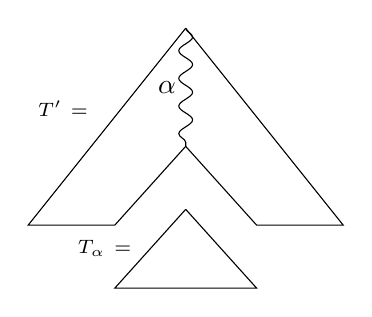
\begin{tikzpicture}
        \coordinate (A) at (0,0);
        \coordinate (B) at (-2,-2.5);
        \coordinate (C) at (2,-2.5);
        \coordinate (D) at (-0.9,-2.5);
        \coordinate (E) at (0.9,-2.5);
        \coordinate (F) at (0,-1.5);
        
        \coordinate (G) at (0,-2.3);
        \coordinate (H) at (-0.9,-3.3);
        \coordinate (I) at (0.9,-3.3);
        
        \draw (A) -- node[above left]{${\scriptstyle T'\ =\ }$}(B) -- (D) -- (F) -- (E) -- (C) -- (A);
        \draw (G) -- node[left]{${\scriptstyle T_\alpha\ =\ }$} (H) -- (I) -- (G);
        
        \draw [photon] (A) -- node[left]{$\alpha$} (F);
      \end{tikzpicture}
      \caption{$T_\alpha = \alpha^{-1}(T)$}
    \end{subfigure}
    $\stackrel{\lambda}{\Rightarrow}$
    \begin{subfigure}[t]{0.5\textwidth}
      \centering
      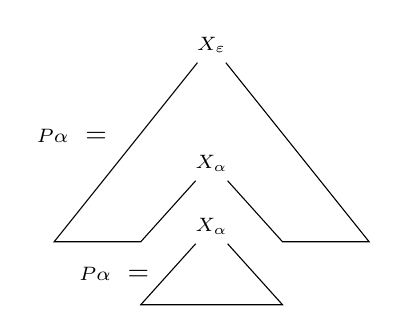
\begin{tikzpicture}
        \node (A) at (0,0) {${\scriptstyle X_\varepsilon}$};
        \coordinate (B) at (-2,-2.5);
        \coordinate (C) at (2,-2.5);
        \coordinate (D) at (-0.9,-2.5);
        \coordinate (E) at (0.9,-2.5);
        \node (F) at (0,-1.5) {${\scriptstyle X_\alpha}$};
        
        \node (G) at (0,-2.3) {${\scriptstyle X_\alpha}$};
        \coordinate (H) at (-0.9,-3.3);
        \coordinate (I) at (0.9,-3.3);
        
        \draw (A) -- node[above left]{${\scriptstyle \uppercut{P}{\alpha}}\ =\ $}(B) -- (D) -- (F) -- (E) -- (C) -- (A);
        \draw (G) -- node[left]{${\scriptstyle \lowercut{P}{\alpha}}\ =\ $} (H) -- (I) -- (G);
      \end{tikzpicture}
      \caption{$\texttt{yield}(\uppercut{P}{\alpha}) = \omega_1 \cdot \texttt{root}(\lowercut{P}{\alpha}) \cdot \omega_2$}
    \end{subfigure}
  \end{figure}
\end{hint}


\subsection*{Най-ляв извод в граматика}
\index{граматика!най-ляв извод}
В нашата дефиниция на извод, изборът върху коя променлива да приложим правило от граматиката е недетерминистичен.
В някои случаи, за нас ще бъде важно винаги да правим детерминистичен избор на това върху коя променлива прилагаме правило.

За две думи $\alpha,\beta \in (V\cup\Sigma)^\star$, дефинираме {\bf най-ляв извод} в граматиката $G$, $\alpha \lderive{\ell} \beta$, по следния начин:
\begin{prooftree}
  \AxiomC{}
  \UnaryInfC{$\alpha \lderive{0} \alpha$}
\end{prooftree}

\begin{prooftree}
  \AxiomC{$A \to_G \gamma$}
  \AxiomC{$\alpha \in \Sigma^\star$}
  \BinaryInfC{$\alpha A \beta \lderive{1} \alpha \gamma \beta$}
\end{prooftree}

\begin{prooftree}
  \AxiomC{$\alpha \lderive{1} \gamma$}
  \AxiomC{$\gamma \lderive{\ell} \beta$}
  \BinaryInfC{$\alpha \lderive{\ell+1} \beta$}
\end{prooftree}

\begin{lemma}
  За всяка безконтекстна граматика $G$, променлива $A \in V$  и дума $\alpha \in (V\cup\Sigma)^\star$,
  \[A \lderive{\star} \alpha\text{ точно тогава, когато } A \derive{\star} \alpha.\]
\end{lemma}
\begin{hint}
  Очевидно е, че ако $A \lderive{\star} \alpha$, то $A \derive{\star} \alpha$.
  За другата посока, достатъчно е да се докаже, че ако $P$ е дърво на извод с корен $A$ и $\texttt{yield}(P) = \alpha$,
  то $A \lderive{\star} \alpha$.

  Индукция по $\texttt{high}(P)$.
\end{hint}



%%% Local Variables:
%%% mode: latex
%%% TeX-master: "../eai"
%%% End:
